% Options for packages loaded elsewhere
\PassOptionsToPackage{unicode}{hyperref}
\PassOptionsToPackage{hyphens}{url}
\documentclass[
  11pt,
  a4paper,
]{article}
\usepackage{xcolor}
\usepackage[margin=22mm]{geometry}
\usepackage{amsmath,amssymb}
\setcounter{secnumdepth}{-\maxdimen} % remove section numbering
\usepackage{iftex}
\ifPDFTeX
  \usepackage[T1]{fontenc}
  \usepackage[utf8]{inputenc}
  \usepackage{textcomp} % provide euro and other symbols
\else % if luatex or xetex
  \usepackage{unicode-math} % this also loads fontspec
  \defaultfontfeatures{Scale=MatchLowercase}
  \defaultfontfeatures[\rmfamily]{Ligatures=TeX,Scale=1}
\fi
\usepackage{lmodern}
\ifPDFTeX\else
  % xetex/luatex font selection
\fi
% Use upquote if available, for straight quotes in verbatim environments
\IfFileExists{upquote.sty}{\usepackage{upquote}}{}
\IfFileExists{microtype.sty}{% use microtype if available
  \usepackage[]{microtype}
  \UseMicrotypeSet[protrusion]{basicmath} % disable protrusion for tt fonts
}{}
\makeatletter
\@ifundefined{KOMAClassName}{% if non-KOMA class
  \IfFileExists{parskip.sty}{%
    \usepackage{parskip}
  }{% else
    \setlength{\parindent}{0pt}
    \setlength{\parskip}{6pt plus 2pt minus 1pt}}
}{% if KOMA class
  \KOMAoptions{parskip=half}}
\makeatother
\usepackage{longtable,booktabs,array}
\newcounter{none} % for unnumbered tables
\usepackage{calc} % for calculating minipage widths
% Correct order of tables after \paragraph or \subparagraph
\usepackage{etoolbox}
\makeatletter
\patchcmd\longtable{\par}{\if@noskipsec\mbox{}\fi\par}{}{}
\makeatother
% Allow footnotes in longtable head/foot
\IfFileExists{footnotehyper.sty}{\usepackage{footnotehyper}}{\usepackage{footnote}}
\makesavenoteenv{longtable}
\usepackage{graphicx}
\makeatletter
\newsavebox\pandoc@box
\newcommand*\pandocbounded[1]{% scales image to fit in text height/width
  \sbox\pandoc@box{#1}%
  \Gscale@div\@tempa{\textheight}{\dimexpr\ht\pandoc@box+\dp\pandoc@box\relax}%
  \Gscale@div\@tempb{\linewidth}{\wd\pandoc@box}%
  \ifdim\@tempb\p@<\@tempa\p@\let\@tempa\@tempb\fi% select the smaller of both
  \ifdim\@tempa\p@<\p@\scalebox{\@tempa}{\usebox\pandoc@box}%
  \else\usebox{\pandoc@box}%
  \fi%
}
% Set default figure placement to htbp
\def\fps@figure{htbp}
\makeatother
\setlength{\emergencystretch}{3em} % prevent overfull lines
\providecommand{\tightlist}{%
  \setlength{\itemsep}{0pt}\setlength{\parskip}{0pt}}
\usepackage{bookmark}
\IfFileExists{xurl.sty}{\usepackage{xurl}}{} % add URL line breaks if available
\urlstyle{same}
\hypersetup{
  pdftitle={Solving Diophantine equations completely: reduction{,} lattices and certificates},
  pdfauthor={GPT-6 Astra (OpenAI), Ultra},
  hidelinks,
  pdfcreator={LaTeX via pandoc}}

\title{Solving Diophantine equations completely: reduction, lattices and
certificates}
\author{GPT-6 Astra (OpenAI), Ultra}
\date{October 2026}

\providecommand{\Eta}{\mathrm{H}}
\begin{document}
\maketitle

\emph{Written by GPT-6 Astra (OpenAI) in Codex, Ultra setting, October
2026. Self-checked by the writing AI. Public domain (CC0).}

A large effective bound and a list of small solutions answer different
questions. The bound limits every possible solution; the list records
what a finite search found. A complete resolution connects them by a
proved reduction and an exhaustive search over the resulting range. This
lesson builds that connection for two exponential equations, and gives
an exact three-logarithm lattice certificate.

We use \href{TR-BAKER-07.html}{\emph{Two logarithms II: explicit
lower bounds}}, Theorem 7.1, for the initial analytic estimate, and
\href{TR-BAKER-11.html}{\emph{Powers of 2 and 3}}, Theorem 11.3 and
equation (11.13), for Legendre's criterion and rational logarithm
intervals. The first equation also reproduces Theorem 11.4 there. The
lattice arguments, reduction lemmas, finite searches and their
certification are proved below.

\subsection{1. From an equation to a finite
certificate}\label{from-an-equation-to-a-finite-certificate}

Suppose an equation yields a nonzero logarithmic form
\(\Lambda=b_1\log\alpha_1+\cdots+b_r\log\alpha_r\) and an upper bound
that decreases exponentially in a size parameter \(X\). An explicit
lower bound for \(|\Lambda|\) first gives \(X\le X_0\). The inequality
may make \(X_0\) too large for direct enumeration. A continued-fraction
calculation or a lattice calculation can then give a much stronger lower
bound for this particular form, throughout the finite coefficient range.
Comparing the two bounds reduces \(X\). Finally one checks every
remaining possibility using exact arithmetic.

Each transition has its own mathematical obligation. The logarithmic
form must be nonzero; the analytic theorem's heights, degree and
coefficient parameter must be correct; the reduction must apply to every
possible coefficient vector; and the last search must exhaust the proved
range. Numerical precision also belongs in the proof: a decimal that
appears positive does not certify a strict inequality.

For two logarithms, division by one of them leads to \(|m-n\theta|\). If
\(m/n=a/b\) in lowest terms and \[
 \left|\theta-\frac mn\right|<\frac1{2n^2},
\] then \(b\le n\), so Legendre's criterion makes \(a/b\) a convergent
of \(\theta\). Writing \(m=ga,n=gb\) gives \[
 |m\log\alpha-n\log\beta|
   =g|a\log\alpha-b\log\beta|,\qquad g\ge1.
\] Thus a lower bound for the reduced convergent's error also bounds the
original error. This common factor is essential when using convergents
to enumerate all possibilities.

An additive term changes the problem to \(u\theta-v+\mu\). The
distance-to-integers argument in the next section handles it. With three
or more logarithms, an integer lattice records several coefficients at
once.

\subsection{2. An inhomogeneous continued-fraction
reduction}\label{an-inhomogeneous-continued-fraction-reduction}

For a real number \(x\), let \(\|x\|=\min_{k\in\mathbb Z}|x-k|\).
Choosing nearest integers proves \(\|x+y\|\le\|x\|+\|y\|\), and, for an
integer \(u\), \(\|ux\|\le |u|\|x\|\). These inequalities are useful
even when the nearest integers are not known individually.

\textbf{Lemma 21.1 (Baker--Davenport reduction).} Let \(M\ge1\) and
\(q\ge1\) be integers, \(\theta,\mu\) real, \(A>0\), and \(B>1\). Put \[
 \epsilon=\|q\mu\|-M\|q\theta\|.
 \tag{21.1}
\] If \(\epsilon>0\), there are no integers \(u,v,w\) satisfying \[
 0<u\le M,\qquad
 0<|u\theta-v+\mu|<AB^{-w},\qquad
 w\ge\frac{\log(Aq/\epsilon)}{\log B}.
 \tag{21.2}
\]

\textbf{Proof.} Multiplication by \(q\), invariance under integer
translation, and the preceding triangle inequality give \[
 \|q\mu\|\le q|u\theta-v+\mu|+u\|q\theta\|
             <qAB^{-w}+M\|q\theta\|.
\] Consequently \(\epsilon<qAB^{-w}\). Taking logarithms and dividing by
the positive number \(\log B\) gives the strict opposite of the last
inequality in (21.2). \(\square\)

In practice \(q\) is a convergent denominator of an irrational
\(\theta\), since this tends to make \(\|q\theta\|\) small. The common
choice \(q>6M\) is a search rule, not a hypothesis used by this proof
and not a guarantee that \(\epsilon>0\). Certified intervals must
establish that strict positivity. The argument also proves the endpoint
exclusion in (21.2), because the small-linear-form inequality is strict.
The author version of
\href{https://web.math.pmf.unizg.hr/~duje/pdf/qjm.pdf}{Dujella and
Pethő, \emph{Generalization of a theorem of Baker and Davenport}}, Lemma
5(a), gives the familiar convergent formulation.

\subsection{3. What an LLL certificate
proves}\label{what-an-lll-certificate-proves}

Let \(z_1,\ldots,z_n\) be linearly independent integer vectors in
\(\mathbb R^n\). Their lattice is \(\Gamma=\sum_i\mathbb Zz_i\). Define
the Gram--Schmidt vectors and coefficients by \[
 z_i^*=z_i-\sum_{j<i}\mu_{ij}z_j^*,\qquad
 \mu_{ij}=\frac{\langle z_i,z_j^*\rangle}{d_j},\qquad
 d_j=\langle z_j^*,z_j^*\rangle>0.
 \tag{21.3}
\] The vectors \(z_i^*\) are mutually orthogonal: taking the inner
product with an earlier \(z_j^*\) cancels exactly its projection term.
Induction also gives equality of the first \(i\) spans. All entries in
(21.3) are rational and can be checked exactly.

A basis is \textbf{LLL reduced with parameter \(3/4\)} if \[
 |\mu_{ij}|\le\tfrac12\quad(j<i),\qquad
 d_i\ge(\tfrac34-\mu_{i,i-1}^2)d_{i-1}\quad(2\le i\le n).
 \tag{21.4}
\]

\textbf{Proposition 21.2 (the shortest-vector guarantee).} An LLL
reduced basis satisfies \[
 \|x\|_2\ge2^{-(n-1)/2}\|z_1\|_2
       \quad(0\ne x\in\Gamma).
 \tag{21.5}
\] For any basis, the possibly stronger certified bound
\(\|x\|_2^2\ge\min_jd_j\) holds.

\textbf{Proof.} Write \(x=\sum_i k_i z_i\), with integers \(k_i\), and
let \(j\) be the largest index with \(k_j\ne0\). Projection on the
orthogonal complement of the first \(j-1\) basis vectors sends \(x\) to
\(k_jz_j^*\). Hence \(\|x\|_2^2\ge k_j^2d_j\ge d_j\), proving the
assertion for an arbitrary basis. Conditions (21.4) give
\(d_i\ge d_{i-1}/2\). Thus
\(d_j\ge2^{-(j-1)}d_1\ge2^{-(n-1)}\|z_1\|_2^2\), which proves (21.5).
\(\square\)

This is the guarantee of
\href{https://www.math.ucdavis.edu/~deloera/MISC/LA-BIBLIO/trunk/Lovasz/LovaszLenstraLenstrafactor.pdf}{Lenstra,
Lenstra and Lovász, \emph{Factoring polynomials with rational
coefficients}}, Proposition (1.11). The computed first vector is an
upper bound for the shortest length; (21.5) supplies the lower bound
needed below.

\textbf{Proposition 21.3 (exact reduction terminates).} Integer row
operations consisting of size reductions and adjacent swaps produce a
basis satisfying (21.4) in finitely many steps.

\textbf{Proof.} Work at an index \(k\), initially two. In decreasing
order of \(j=k-1,\ldots,1\), replace \(z_k\) by \(z_k-rz_j\), where
\(r\) is a nearest integer to the current \(\mu_{kj}\). This makes
\(|\mu_{kj}|\le1/2\); later reductions with smaller indices do not
change it. The operation preserves the integer lattice, and its inverse
adds \(rz_j\). If the adjacent inequality in (21.4) holds, increase
\(k\). Otherwise exchange \(z_{k-1},z_k\) and restart at
\(\max\{2,k-1\}\). Terminate when \(k=n+1\). At each stage the earlier
prefix is reduced; hence termination gives all of (21.4).

Here is a decreasing integer that proves termination. Put \[
 D_i=\det(\langle z_r,z_s\rangle_{r,s\le i})
      =\prod_{j=1}^i d_j,\qquad
 \mathcal P=\prod_{i=1}^{n-1}D_i.
 \tag{21.6}
\] The determinant identity follows by the triangular Gram--Schmidt
change of basis, whose determinant is one. Each \(D_i\) is a positive
integer. Size reductions preserve every prefix lattice and hence every
\(D_i\). A swap at \(k\) preserves every factor except \(D_{k-1}\).
Projecting the new \((k-1)\)-st vector on the orthogonal complement of
the first \(k-2\) vectors shows that the ratio of the new factor to the
old is \[
 \frac{d_k+\mu_{k,k-1}^2d_{k-1}}{d_{k-1}}<\frac34.
\] Thus each swap reduces the positive integer \(\mathcal P\) by a
factor below \(3/4\). There are finitely many swaps. Between swaps the
index increases after finitely many size reductions, so the entire
algorithm terminates. For \(n=1\) there is nothing to do. \(\square\)

For a certificate, record the integer change-of-basis matrix as well as
the output basis. A determinant of \(\pm1\) and the exact basis identity
certify equality of lattices. Exact values of the rational \(\mu_{ij}\)
and \(d_i\) then certify (21.4). No floating-point claim of ``LLL
reduced'' is needed.

\subsection{4. A lattice lower bound for a logarithmic
form}\label{a-lattice-lower-bound-for-a-logarithmic-form}

\textbf{Lemma 21.4 (de Weger-type reduction).} Let \(\alpha_j>0\),
\(C>0\), \(X_0\ge0\), and \(b_j\in\mathbb Z\) with \(|b_j|\le X_0\), not
all zero. Set \(\Lambda=\sum_jb_j\log\alpha_j\). Let \(A_C\) be the
integer matrix whose first \(n-1\) rows are the corresponding rows of
the identity matrix and whose last row is
\((\lfloor C\log\alpha_1\rfloor,\ldots,
\lfloor C\log\alpha_n\rfloor)\). Suppose \(A_C\) is nonsingular and
every nonzero vector of \(\Gamma=A_C\mathbb Z^n\) has Euclidean norm at
least \(l_0\). If \(l_0^2>(n-1)X_0^2\), then \[
 C|\Lambda|\ge
 \sqrt{l_0^2-(n-1)X_0^2}-nX_0.
 \tag{21.7}
\]

\textbf{Proof.} The vector \(A_Cb\) is nonzero by nonsingularity. Its
first \(n-1\) coordinates are \(b_1,\ldots,b_{n-1}\); write its last
coordinate as \(s\). Thus \(l_0^2\le\|A_Cb\|_2^2\le(n-1)X_0^2+s^2\),
giving the square-root lower bound for \(|s|\). On the other hand, \[
 |s-C\Lambda|
 \le\sum_j|b_j|\,
       |\lfloor C\log\alpha_j\rfloor-C\log\alpha_j|
 \le nX_0.
\] The ordinary triangle inequality now proves (21.7). \(\square\)

The determinant of \(A_C\) is \(\lfloor C\log\alpha_n\rfloor\). Thus
\(\alpha_n\ne1\) alone does not certify nonsingularity for an
arbitrarily small \(C\); check the actual integer. Also, the right side
of (21.7) must be positive before it gives useful information. The
sufficient condition is \(l_0^2>(n^2+n-1)X_0^2\).

\textbf{Corollary 21.5 (combining the two directions).} Suppose in
addition that \(0<|\Lambda|<A\exp(-\lambda X)\), with \(A,\lambda>0\),
and that the right side \(E\) of (21.7) is positive. Then \[
 X<\frac{\log(AC/E)}{\lambda}.
 \tag{21.8}
\]

\textbf{Proof.} We have \(0<E/C\le|\Lambda|<A\exp(-\lambda X)\). Take
logarithms and rearrange. \(\square\)

The small upper bound comes from the original Diophantine equation. A
bound \(|b_j|\le X_0\) by itself does not imply a smaller bound for the
coefficients. The lattice supplies a lower bound for the linear form,
which must be compared with that additional upper bound.

\subsection{5. Two complete exponential
resolutions}\label{two-complete-exponential-resolutions}

All exponents in this section are positive integers. We resolve \[
 |2^m-3^n|\le20,\qquad |2^m-5^n|\le20.
 \tag{21.9}
\] The first calculation reproduces the earlier continued-fraction
certificate; the second uses the same steps with different exact data.
In both cases unique prime factorization ensures that the two powers are
unequal and that their logarithmic form is nonzero.

\subsubsection{5.1. The powers of two and
three}\label{the-powers-of-two-and-three}

\textbf{Theorem 21.6.} All solutions of the first inequality in (21.9)
are \[
\begin{array}{c|l}
n&\text{allowed }m\\ \hline
1&1,2,3,4\\
2&1,2,3,4\\
3&3,4,5\\
4&6\\
5&8
\end{array}
\tag{21.10}
\] There are no solutions with \(n\ge6\).

\textbf{Proof: initial bound.} For \(n\ge4\), the argument of Theorem
11.4 gives \(m\ge6\), \(n<m\), and \[
 0<|m\log2-n\log3|<30\,2^{-m}.
\] For completeness, \(2^m\ge3^4-20=61\); if \(n\ge m\), then
\(3^n-2^m\ge3^m-2^m>20\). For positive \(x,y\), integration gives
\(|\log x-\log y|\le |x-y|/\min(x,y)\). Apply this with \(x=2^m,y=3^n\)
and use \(20/2^m\le5/16\). The resulting constant is
\(20/(1-5/16)=320/11<30\).

Theorem 7.1 with field degree one, height parameters
\(a_1=1,a_2=\log3\), and coefficients \(m,-n\), gives \[
 m\log2<\log30+
 21600\log3\bigl(\max\{10,\log(2m)\}\bigr)^2.
 \tag{21.11}
\] Indeed \(h(2)=\log2<1\), \(h(3)=\log3>1\), and the theorem's
coefficient parameter is \(m/\log3+n<2m\). For \(x\ge10^7\), set \[
 F_3(x)=x\log2-21600\log3\log^2(2x)-\log30.
\] The rational bounds
\(\log2>69/100,\ \log3<11/10,\ \log(2\cdot10^7)<17,\ \log30<4\) give
\(F_3(10^7)>33356>0\). Also \(\log(2x)/x\) decreases there, and hence \[
 F_3'(x)>
 \frac{69}{100}-\frac{43200(11/10)17}{10^7}
 =\frac{9519}{15625}>0.
\] The maximum in (21.11) equals \(\log(2x)\) on this range. Therefore
\(m<10^7\).

\textbf{Proof: reduction.} For \(n\ge6\), \[
 \left|\frac{\log3}{\log2}-\frac mn\right|
 \le\frac{20}{n\log2(3^n-20)}<\frac1{2n^2}.
 \tag{21.12}
\] The last inequality holds at six because
\((69/100)(3^6-20)>40\cdot6\). The quantity \((3^n-20)/n\) increases:
the numerator of its successive difference is \((2n-1)3^n+20>0\).
Legendre therefore applies to \(a/b=m/n\) in lowest terms, and the
reduced numerator satisfies \(a<10^7\).

The table lists every eligible convergent and the first excluded one.
The sign is that of \(p_j\log2-q_j\log3\), and each integer \(L_j\)
satisfies \(10^8|p_j\log2-q_j\log3|>L_j\).

{\def\LTcaptype{none} % do not increment counter
\begin{longtable}[]{@{}rrrrrr@{}}
\toprule\noalign{}
\(j\) & \(a_j\) & \(p_j\) & \(q_j\) & sign & \(L_j\) \\
\midrule\noalign{}
\endhead
\bottomrule\noalign{}
\endlastfoot
0 & 1 & 1 & 1 & \(-\) & 40546510 \\
1 & 1 & 2 & 1 & + & 28768207 \\
2 & 1 & 3 & 2 & \(-\) & 11778303 \\
3 & 2 & 8 & 5 & + & 5211600 \\
4 & 2 & 19 & 12 & \(-\) & 1355103 \\
5 & 3 & 65 & 41 & + & 1146290 \\
6 & 1 & 84 & 53 & \(-\) & 208813 \\
7 & 5 & 485 & 306 & + & 102223 \\
8 & 2 & 1054 & 665 & \(-\) & 4365 \\
9 & 23 & 24727 & 15601 & + & 1819 \\
10 & 2 & 50508 & 31867 & \(-\) & 726 \\
11 & 2 & 125743 & 79335 & + & 366 \\
12 & 1 & 176251 & 111202 & \(-\) & 360 \\
13 & 1 & 301994 & 190537 & + & 6 \\
14 & 55 & 16785921 & 10590737 & \(-\) & 5 \\
\end{longtable}
}

All rows before the last have \(L_j\ge1\), and subsequent numerators are
larger still. Multiplication by the common factor \(g\ge1\) does not
decrease the error. Thus \[
 |m\log2-n\log3|>10^{-8}.
 \tag{21.13}
\] Together with the upper bound \(20/(3^n-20)\), this gives
\(3^n<2000000020\). Since \(3^{20}=3486784401\), every solution has
\(n\le19\). Cases below six are checked separately below.

For \(6\le n\le19\), let \(k=\lfloor\log_2(3^n)\rfloor\). The following
exact integers give the distances to the powers on either side of
\(3^n\).

{\def\LTcaptype{none} % do not increment counter
\begin{longtable}[]{@{}rrrr@{}}
\toprule\noalign{}
\(n\) & \(k\) & \(3^n-2^k\) & \(2^{k+1}-3^n\) \\
\midrule\noalign{}
\endhead
\bottomrule\noalign{}
\endlastfoot
6 & 9 & 217 & 295 \\
7 & 11 & 139 & 1909 \\
8 & 12 & 2465 & 1631 \\
9 & 14 & 3299 & 13085 \\
10 & 15 & 26281 & 6487 \\
11 & 17 & 46075 & 84997 \\
12 & 19 & 7153 & 517135 \\
13 & 20 & 545747 & 502829 \\
14 & 22 & 588665 & 3605639 \\
15 & 23 & 5960299 & 2428309 \\
16 & 25 & 9492289 & 24062143 \\
17 & 26 & 62031299 & 5077565 \\
18 & 28 & 118985033 & 149450423 \\
19 & 30 & 88519643 & 985222181 \\
\end{longtable}
}

Every distance exceeds twenty. Every other power is farther away, so
this excludes the whole range. For \(1\le n\le5\), enumerate every
positive \(m\) with \(2^m\le3^n+20\), which is a finite integer test.
The successful values are exactly (21.10). Their signed differences
\(2^m-3^n\), in the order shown, are \[
 (-1,1,5,13),\quad(-7,-5,-1,7),\quad(-19,-11,5),\quad-17,\quad13.
\] The full small-exponent search, including its excluded entries, is
recorded in the certificate. This proves the theorem. \(\square\)

\subsubsection{5.2. The powers of two and
five}\label{the-powers-of-two-and-five}

\textbf{Theorem 21.7.} All solutions of the second inequality in (21.9)
are \[
\begin{array}{c|l}
n&\text{allowed }m\\ \hline
1&1,2,3,4\\
2&3,4,5\\
3&7
\end{array}
\tag{21.14}
\] There are no solutions with \(n\ge4\).

\textbf{Proof: initial bound.} Suppose first that \(n\ge3\). Then
\(2^m\ge125-20=105\), so \(m\ge7\). If \(n\ge m\), then
\(5^n-2^m\ge5^m-2^m>20\), a contradiction. Put
\(\Lambda=m\log2-n\log5\ne0\). Integration as above gives \[
 |\Lambda|\le\frac{20}{2^m-20}
 \le\frac{640}{27}\,2^{-m}<24\,2^{-m}.
 \tag{21.15}
\] The middle inequality uses \(20/2^m\le5/32\). Apply Theorem 7.1 with
\(D=1\), \(a_1=1\), \(a_2=\log5\). The height conditions hold, and
\(B'=m/\log5+n<2m\). Consequently \[
 m\log2<\log24+
 21600\log5\bigl(\max\{10,\log(2m)\}\bigr)^2.
 \tag{21.16}
\] This implies \(m<2\cdot10^7\). To check the entire excluded interval,
define \(F_5(x)=x\log2-21600\log5\log^2(2x)-\log24\). Use
\(\log5<17/10\), \(\log(4\cdot10^7)<18\) and \(\log24<4\). At
\(x=2\cdot10^7\) these give \[
 F_5(x)>1902716,\qquad
 F_5'(x)>\frac{69}{100}
 -\frac{43200(17/10)18}{2\cdot10^7}
 =\frac{19497}{31250}>0.
\] As before, \(\log(2x)/x\) decreases, so the derivative remains
positive. The maximum in (21.16) is \(\log(2x)\) throughout this
interval. Thus (21.16) is impossible there.

\textbf{Proof: reduction.} For \(n\ge4\), \[
 \left|\frac{\log5}{\log2}-\frac mn\right|
 \le\frac{20}{n\log2(5^n-20)}<\frac1{2n^2}.
 \tag{21.17}
\] At four the last inequality follows from
\((69/100)(5^4-20)>40\cdot4\). The numerator of the successive
difference of \((5^n-20)/n\) is \((4n-1)5^n+20>0\), so the inequality
persists. The reduced fraction \(a/b=m/n\) is therefore a convergent of
\(\log5/\log2\), with \(a<2\cdot10^7\).

The following table has the same meaning as before, with
\(L_j<10^8|p_j\log2-q_j\log5|\).

{\def\LTcaptype{none} % do not increment counter
\begin{longtable}[]{@{}rrrrrr@{}}
\toprule\noalign{}
\(j\) & \(a_j\) & \(p_j\) & \(q_j\) & sign & \(L_j\) \\
\midrule\noalign{}
\endhead
\bottomrule\noalign{}
\endlastfoot
0 & 2 & 2 & 1 & \(-\) & 22314355 \\
1 & 3 & 7 & 3 & + & 2371652 \\
2 & 9 & 65 & 28 & \(-\) & 969481 \\
3 & 2 & 137 & 59 & + & 432690 \\
4 & 2 & 339 & 146 & \(-\) & 104100 \\
5 & 4 & 1493 & 643 & + & 16288 \\
6 & 6 & 9297 & 4004 & \(-\) & 6372 \\
7 & 2 & 20087 & 8651 & + & 3544 \\
8 & 1 & 29384 & 12655 & \(-\) & 2828 \\
9 & 1 & 49471 & 21306 & + & 716 \\
10 & 3 & 177797 & 76573 & \(-\) & 679 \\
11 & 1 & 227268 & 97879 & + & 36 \\
12 & 18 & 4268621 & 1838395 & \(-\) & 31 \\
13 & 1 & 4495889 & 1936274 & + & 4 \\
14 & 6 & 31243955 & 13456039 & \(-\) & 3 \\
\end{longtable}
}

The last numerator exceeds \(2\cdot10^7\); every earlier row has
\(L_j\ge1\). The same common-factor argument gives
\(|\Lambda|>10^{-8}\). Hence \(5^n<2000000020\), and \[
 5^{14}=6103515625>2000000020
 \quad\Longrightarrow\quad n\le13.
 \tag{21.18}
\] For \(4\le n\le13\), the exact nearest-power distances are:

{\def\LTcaptype{none} % do not increment counter
\begin{longtable}[]{@{}rrrr@{}}
\toprule\noalign{}
\(n\) & \(k\) & \(5^n-2^k\) & \(2^{k+1}-5^n\) \\
\midrule\noalign{}
\endhead
\bottomrule\noalign{}
\endlastfoot
4 & 9 & 113 & 399 \\
5 & 11 & 1077 & 971 \\
6 & 13 & 7433 & 759 \\
7 & 16 & 12589 & 52947 \\
8 & 18 & 128481 & 133663 \\
9 & 20 & 904549 & 144027 \\
10 & 23 & 1377017 & 7011591 \\
11 & 25 & 15273693 & 18280739 \\
12 & 27 & 109922897 & 24294831 \\
13 & 30 & 146961301 & 926780523 \\
\end{longtable}
}

All entries exceed twenty. For \(n=1,2,3\), check every \(m\ge1\) with
\(2^m\le5^n+20\); the upper endpoints for \(m\) are respectively four,
five and seven. The successful differences are \[
 (-3,-1,3,11),\qquad(-17,-9,7),\qquad3,
\] giving exactly (21.14). \(\square\)

\subsubsection{5.3. Why the numerical tables are
proofs}\label{why-the-numerical-tables-are-proofs}

For a rational \(x>1\), put \(z=(x-1)/(x+1)\). The positive series and
geometric remainder proved in (11.13) give \[
 L_N(x)=2\sum_{j=0}^{N-1}\frac{z^{2j+1}}{2j+1},
 \qquad
 L_N(x)<\log x<
 L_N(x)+\frac{2z^{2N+1}}{(2N+1)(1-z^2)}=U_N(x).
 \tag{21.19}
\] Use \(N=100\) for \(x=2,3,5\). Start the continued-fraction
calculation with the interval \[
 [L_N(p)/U_N(2),U_N(p)/L_N(2)].
\] At each step both endpoints have the same integer part. Subtract that
integer and invert the interval, reversing its endpoints. This certifies
every partial quotient in the two tables.

The error interval for a row \(a,b\) is
\([aL_N(2)-bU_N(p),aU_N(2)-bL_N(p)]\). It lies strictly on one side of
zero. Multiplying its distance from zero by \(10^8\) and taking the
integer part produces the printed \(L_j\). The recurrence
\(p_j=a_jp_{j-1}+p_{j-2}\), \(q_j=a_jq_{j-1}+q_{j-2}\), with
\((p_{-2},p_{-1})=(0,1)\) and \((q_{-2},q_{-1})=(1,0)\), gives all table
entries. Their determinant identities \(|p_jq_{j-1}-p_{j-1}q_j|=1\) are
also checked.

For the scalar logarithm bounds, (21.19) certifies
\(69/100<\log2<7/10\), \(1<\log3<11/10\) and \(1<\log5<17/10\). Positive
exponential partial sums give \[
 \sum_{j=0}^{80}\frac{17^j}{j!}>2\cdot10^7,\qquad
 \sum_{j=0}^{80}\frac{18^j}{j!}>4\cdot10^7,\qquad
 \sum_{j=0}^{12}\frac{4^j}{j!}>30.
\] These are finite rational comparisons. Also
\(2x\ge2\cdot10^7>2^{20}\) at either initial endpoint, so
\(\log(2x)>20(69/100)>10\). No floating-point estimate is used to
certify these inequalities.

The \href{verification/equation-certificates.py}{equation certificate
program} reconstructs the intervals, convergents, analytic margins and
final integer searches. Its
\href{verification/equation-certificates.json}{machine-readable data}
include all successful and unsuccessful small-exponent tests. The
preceding proofs explain why those finite tests settle (21.9) for
arbitrarily large positive exponents.

\subsection{\texorpdfstring{6. A three-logarithm certificate from
\(10^{20}\)}{6. A three-logarithm certificate from 10\^{}\{20\}}}\label{a-three-logarithm-certificate-from-1020}

Consider \[
 \Lambda=b_1\log2+b_2\log3+b_3\log5,\qquad
 0<X=\max_j|b_j|\le X_0=10^{20}.
 \tag{21.20}
\] We first bound \(|\Lambda|\) uniformly on this coefficient range.
Then we show precisely what follows if the equation under study also
gives \(|\Lambda|<e^{-X}\).

Choose \(C=10^{70}\), and put \(N_p=\lfloor C\log p\rfloor\). The
following expressions give each integer exactly, split into two blocks
of decimal digits:

\[
\begin{aligned}
N_2={}&69314718055994530941723212145817656\cdot10^{35}\\
&+80755001343602552541206800094933936.
\end{aligned}
\]

\[
\begin{aligned}
N_3={}&109861228866810969139524523692252570\cdot10^{35}\\
&+46474905578227494517346943336374942.
\end{aligned}
\]

\[
\begin{aligned}
N_5={}&160943791243410037460075933322618763\cdot10^{35}\\
&+95256013542685177219126478914741789.
\end{aligned}
\]

These floors are certified as follows. For \(p=2,3,5\), write
\(p=2^k y\) with \(1\le y<2\). Use (21.19) with 240 terms for \(\log2\)
and \(\log y\), and add \(k\) times the former interval to the latter.
If \(y=1\), its interval is exactly zero. The resulting rational
interval \([\ell_p,u_p]\) satisfies \[
 N_p\le C\ell_p<C u_p<N_p+1
 \quad(p=2,3,5).
 \tag{21.21}
\] Both endpoints are given as exact rational numbers in the
\href{verification/reduction-lattice-check.json}{lattice certificate
data}. The certified floors, rather than rounded decimal logarithms, are
the integers used in the lattice.

Take the matrix \[
 A_C=
 \begin{pmatrix}
 1&0&0\\0&1&0\\N_2&N_3&N_5
 \end{pmatrix}.
\] Its determinant is \(N_5>0\). For the reduction calculation we store
its column generators as the rows of \(B=A_C^{\mathsf T}\). Integer row
operations give the following reduced basis. Each displayed tuple is a
row of \(Z\).

\[
\begin{aligned}
z_1={}&\bigl(-113787772450244355120783,\ 128201904809150744170883,\\
&\phantom{(}\ -115968960281991971372137\bigr).
\end{aligned}
\]

\[
\begin{aligned}
z_2={}&\bigl(25526442133869073534457,\ -46145588766202269201100,\\
&\phantom{(}\ -245168407442614588037248\bigr).
\end{aligned}
\]

\[
\begin{aligned}
z_3={}&\bigl(-307703996139997391582989,\ -152884949282210989518165,\\
&\phantom{(}\ 29629247620621709800972\bigr).
\end{aligned}
\]

To certify that these vectors generate the original lattice, use the
integer matrix \(U\) with the following rows.

\[
\begin{aligned}
\operatorname{row}_1(U)={}&\bigl(-113787772450244355120783,\ 128201904809150744170883,\\
&\phantom{(}\ -38505688177919229524815\bigr).
\end{aligned}
\]

\[
\begin{aligned}
\operatorname{row}_2(U)={}&\bigl(25526442133869073534457,\ -46145588766202269201100,\\
&\phantom{(}\ 20505624501938193115800\bigr).
\end{aligned}
\]

\[
\begin{aligned}
\operatorname{row}_3(U)={}&\bigl(-307703996139997391582989,\ -152884949282210989518165,\\
&\phantom{(}\ 236881111386715610374554\bigr).
\end{aligned}
\]

Direct integer multiplication gives \(Z=UB\), and \(\det U=1\). Thus
\(U\) and its inverse have integer entries and the two sets of rows
generate exactly the same lattice. The inverse is integral because the
adjugate identity expresses it as the integer adjugate divided by
\(\det U=1\).

The rational Gram--Schmidt calculation (21.3) on \(Z\) satisfies all
three inequalities \(|\mu_{ij}|\le1/2\) and both Lovász inequalities
(21.4). The
\href{verification/reduction_lattice_certificate.py}{exact reduction
program} records the rational numerators and denominators for each of
these checks. It also replays every integer row operation: there are 126
nonzero size reductions and 110 swaps. Each reduction preserves the
integer potential (21.6), and each swap decreases it by a factor
strictly below \(3/4\). These checks give both a reproducible
construction and a certificate of the final basis. The final basis
identity and inequalities alone are sufficient to use Proposition 21.2.

\textbf{Proposition 21.8.} Every coefficient vector in (21.20) satisfies
\[
 |\Lambda|>10^{-48}.
 \tag{21.22}
\] If, in addition, \(0<|\Lambda|<e^{-X}\), then \[
 X\le119.
 \tag{21.23}
\]

\textbf{Proof.} Proposition 21.2 with \(n=3\) permits \[
 l_0^2=\frac{\|z_1\|_2^2}{4}
 =\frac{42832185304769368334706960617223635440163479547}{4}.
\] Let \[
 R=103479593767043471534146,\qquad
 E_0=R-3\cdot10^{20}=103179593767043471534146.
\] Exact squaring gives \[
 R^2\le l_0^2-2\cdot10^{40}<(R+1)^2.
\] Therefore the square root in (21.7), minus the rounding error
\(3X_0\), is at least \(E_0>0\). Lemma 21.4 now gives \[
 C|\Lambda|\ge E_0,\qquad E_0\,10^{48}>10^{70}=C,
\] which proves (21.22). If the additional upper bound holds and
\(X\ge120\), then \[
 |\Lambda|<e^{-X}\le e^{-120}<10^{-48},
\] a contradiction. For the last strict comparison,
\(e>1+1+1/2+1/6=8/3\), and the integer comparison
\(8^{120}>10^{48}3^{120}\) proves \((8/3)^{120}>10^{48}\). Thus
\(X<120\), giving (21.23) because \(X\) is an integer. \(\square\)

The condition \(0<|\Lambda|<e^{-X}\) is an explicit assumption in the
second conclusion. A coefficient bound alone cannot imply that all
coefficients are small: for example \((b_1,b_2,b_3)=(10^{20},0,0)\)
belongs to the initial box. For another Diophantine problem its own
upper bound \(A e^{-\lambda X}\) can instead be inserted in (21.8).

The matrix construction and comparison of its last coordinate with the
logarithmic form are the mechanism used in
\href{https://math.deweger.net/proefschrift/proefschrift-hoofdstuk3.pdf}{de
Weger, \emph{Algorithms for Diophantine Equations}, original doctoral
thesis}, Section 3.7, Lemma 3.7 and equation (3.23), printed pages
57--59. Here the horizontal scale is one, all rounding is downward, and
Lemma 21.4 keeps the square-root expression explicit.

\begin{minipage}[t]{\linewidth}
\centering
\pandocbounded{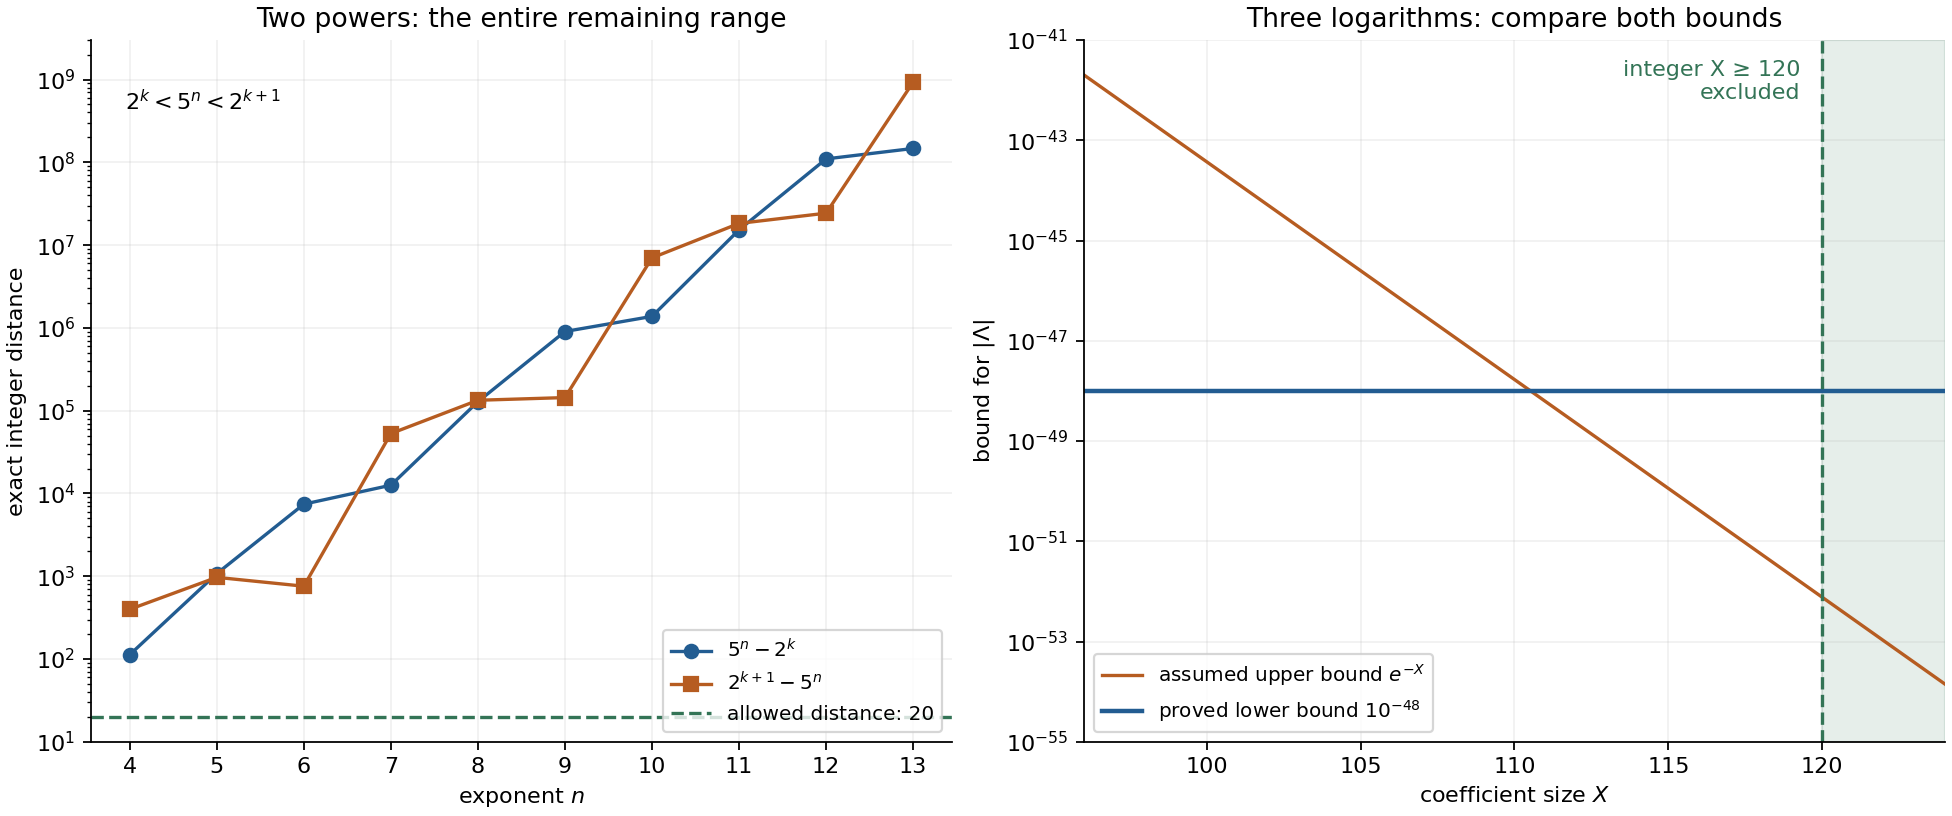
\includegraphics[keepaspectratio,alt={Certified logarithmic-form bounds for two complete equations and a three-logarithm lattice}]{../figures/reduction-certificates.png}}
\par\smallskip
\begin{flushleft}\small
\emph{Figure 21.1. Left: exact distances from \(5^n\) to the adjacent
powers of two for \(4\le n\le13\); the entire interval is excluded by
Theorem 21.7. The horizontal dashed line is the allowed distance 20.
Right: the proved lattice lower bound \(10^{-48}\) and the additional
upper bound \(e^{-X}\), displayed on a logarithmic vertical scale. The
sampled curve illustrates Proposition 21.8; the exclusion at integer
\(X=120\) is proved by the exact comparison \(8^{120}>10^{48}3^{120}\),
not by the plot.
\href{figure_sources/reduction_certificate_figure.py}{Figure
program}.}
\end{flushleft}
\end{minipage}\par\medskip


\subsection{7. Exercises and complete
solutions}\label{exercises-and-complete-solutions}

\begin{enumerate}
\def\labelenumi{\arabic{enumi}.}
\tightlist
\item
  \textbf{Easy: the distance lemma.} Prove Lemma 21.1 directly.
  Determine whether a convergent hypothesis, \(q>6M\), or a strict
  exclusion threshold for \(w\) is necessary.
\item
  \textbf{Medium: a homogeneous certificate.} Implement the
  continued-fraction reduction for \(m\log2-n\log3\) using rational
  arithmetic. Reproduce the convergents and the final range of Theorem
  11.4. Explain why reducing \(m/n\) to lowest terms loses no solutions,
  and resolve the positive exponents with \(n<4\).
\item
  \textbf{Medium: the lattice lemma.} Prove (21.7). Identify the precise
  purpose of nonsingularity and give a sufficient condition for its
  right side to be positive.
\item
  \textbf{Hard: an exact LLL reduction.} For the form in (21.20), start
  from \(X_0=10^{20}\), choose \(C\), and certify a lattice lower bound.
  Assuming also \(0<|\Lambda|<e^{-X}\), reduce the coefficient range.
  Record enough exact information to reconstruct every rounding and
  every basis operation.
\end{enumerate}

\textbf{Solution 1.} Let \(t\in\mathbb Z\) be nearest to \(q\theta\).
The identity \[
 q\mu=q(u\theta-v+\mu)-u(q\theta-t)+(qv-ut)
\] has integer final term. Taking distance to the integers gives \[
 \|q\mu\|\le q|u\theta-v+\mu|+u\|q\theta\|
 <qAB^{-w}+M\|q\theta\|.
\] Thus \(\epsilon<qAB^{-w}\). If \(w\ge\log(Aq/\epsilon)/\log B\), then
\(qAB^{-w}\le\epsilon\), a contradiction. Neither a convergent nor
\(q>6M\) was used. The endpoint is excluded because the original upper
bound is strict. The essential numerical condition is \(\epsilon>0\); if
it fails, this argument gives no exclusion.

\textbf{Solution 2.} Compute the two intervals (21.19) with \(N=100\).
Apply integer-part extraction and reversed reciprocal intervals to their
ratio. Starting from the four recurrence values in Section 5.3, the
partial quotients through the first excluded numerator are \[
 1,1,1,2,2,3,1,5,2,23,2,2,1,1,55.
\] The last eligible numerator and denominator are \(301994,190537\);
the next pair is \(16785921,10590737\), so its numerator violates the
proved strict bound \(m<10^7\). The least printed \(L_j\) among eligible
rows is six, which is more than needed for the uniform error
\(10^{-8}\). For \(m=gp,n=gq\), the logarithmic form is \(g\) times the
reduced error. Since \(g\ge1\), the uniform lower bound remains valid.
The upper bound \(20/(3^n-20)\) then gives \(n\le19\). Exact integer
comparisons for \(4\le n\le19\) yield only \((m,n)=(6,4),(8,5)\). For
\(n=1,2,3\), enumerate \(1\le m\le
\lfloor\log_2(3^n+20)\rfloor\), using integer bit lengths. The
successful sets are respectively \(\{1,2,3,4\}\), \(\{1,2,3,4\}\) and
\(\{3,4,5\}\), as in (21.10). The linked equation program implements
these operations with integers and fractions and checks every printed
convergent.

\textbf{Solution 3.} Put \(v=A_Cb\) and write its last coordinate as
\(s=\sum b_j\lfloor C\log\alpha_j\rfloor\). Nonsingularity and \(b\ne0\)
ensure \(v\ne0\), so \[
 l_0^2\le\|v\|_2^2
 =\sum_{j<n}b_j^2+s^2
 \le(n-1)X_0^2+s^2.
\] The hypothesis makes the resulting lower bound
\(|s|\ge\sqrt{l_0^2-(n-1)X_0^2}\) real and positive. Each floor
introduces an error less than one, hence \(|s-C\Lambda|\le nX_0\).
Subtract this error using the triangle inequality to obtain (21.7). Its
right side is positive exactly when \(l_0^2>(n^2+n-1)X_0^2\). The weaker
displayed hypothesis in Lemma 21.4 is enough for the inequality, but may
leave a nonpositive lower bound.

\textbf{Solution 4.} Choose \(C=10^{70}\). The 240-term intervals in
Section 6 certify all three floors and hence the integer matrix \(A_C\).
Execute size reductions using nearest integers to the exact
Gram--Schmidt fractions, and swap only when the exact Lovász inequality
fails. Carry the same row operations on the identity matrix to obtain
\(U\). The program records 236 operations, including 110 swaps, and
verifies every potential comparison. Its output is the displayed basis
\(Z\) and \(\det U=1\). Check \(Z=UA_C^{\mathsf T}\), the three size
inequalities, and the two Lovász inequalities. Proposition 21.2 gives
\(l_0^2=\|z_1\|^2/4\). The exact square-root bracket in Proposition 21.8
then gives \(C|\Lambda|\ge103179593767043471534146>C10^{-48}\). The
assumed upper bound rules out \(X\ge120\), since
\(8^{120}>10^{48}3^{120}\) and \(e>8/3\). Thus the reduced integer bound
is \(X\le119\). Without the additional upper bound the certified
conclusion is \(|\Lambda|>10^{-48}\), not a smaller coefficient range.

\subsection{8. What to retain with a complete
resolution}\label{what-to-retain-with-a-complete-resolution}

A reproducible certificate has four connected parts:

\begin{enumerate}
\def\labelenumi{\arabic{enumi}.}
\tightlist
\item
  The equation, domain, logarithmic form and proof of nonvanishing,
  followed by the exact analytic theorem, its parameters and the
  resulting initial bound.
\item
  Rational logarithm intervals, their remainder estimates, and either
  all required convergents or the integer lattice matrix, change of
  basis and rational Gram--Schmidt checks.
\item
  The comparison proving the reduced bound, with strict endpoints and
  common factors handled explicitly.
\item
  The exhaustive integer search range and its complete output, including
  the small cases excluded from earlier inequalities.
\end{enumerate}

For the two equations, the certificate data contain all these finite
checks and the proofs above supply the analytic implications. For the
lattice example, the data also contain every elementary operation and
the positive integer potential that decreases at swaps. All programs use
the Python standard library for their proof checks. The figure uses
numerical coordinates only to illustrate inequalities already proved
exactly.

\subsubsection{What this lesson uses from earlier
lessons}\label{what-this-lesson-uses-from-earlier-lessons}

Theorem 7.1 supplies the explicit two-logarithm lower bound with
constant \(21600\). Theorem 11.3 supplies Legendre's criterion, and
equation (11.13) supplies the rational logarithm intervals. These
results are proved in the linked earlier lessons. Theorem 11.4 is
reproduced here, including its finite reduction. No external citation
replaces a reduction proof or a search exhaustiveness argument in this
lesson.

\subsubsection{Freely accessible
sources}\label{freely-accessible-sources}

\begin{itemize}
\tightlist
\item
  A. Dujella and A. Pethő, \emph{Generalization of a theorem of Baker
  and Davenport}, Lemma 5(a),
  \href{https://web.math.pmf.unizg.hr/~duje/pdf/qjm.pdf}{author
  version}.
\item
  A. K. Lenstra, H. W. Lenstra, Jr., and L. Lovász, \emph{Factoring
  polynomials with rational coefficients}, Section 1, especially
  Proposition (1.11),
  \href{https://www.math.ucdavis.edu/~deloera/MISC/LA-BIBLIO/trunk/Lovasz/LovaszLenstraLenstrafactor.pdf}{free
  university-hosted paper}.
\item
  B. M. M. de Weger, \emph{Algorithms for Diophantine Equations},
  original doctoral thesis (1988), Chapter 3, Section 3.7,
  \href{https://math.deweger.net/proefschrift/proefschrift-hoofdstuk3.pdf}{free
  author-hosted chapter}.
\end{itemize}

\end{document}
